\documentclass[12pt]{article}
\usepackage[utf8]{inputenc}
\usepackage[spanish]{babel}
\usepackage{amsmath, amssymb}
\usepackage{graphicx}
\usepackage{geometry}
\usepackage{booktabs}
\usepackage{float}
\usepackage{hyperref}
\usepackage[backend=biber, sorting=none]{biblatex}
\addbibresource{./references/references.bib}

\geometry{margin=1in}
\setlength{\parskip}{1em}
\setlength{\parindent}{0pt}

\title{Simulación y Análisis de Sistemas de Colas en una Sucursal Bancaria}
\author{Jorge Alejandro Echevarría Brunet}
\date{\today}

\begin{document}

\maketitle

\newpage

\tableofcontents

\newpage

\section{Introducción}\label{sec:introduccion}
Este proyecto analiza, mediante simulación de eventos discretos, dos configuraciones operativas en una pequeña sucursal bancaria. En el sistema actual, dos empleados atienden de forma especializada: uno se encarga de pagos y otro de cobros, cada uno con su propia cola independiente. La propuesta consiste en que ambos empleados sean polivalentes y atiendan una única cola, lo que podría evitar la situación en la que una cola se encuentre saturada mientras la otra permanece inactiva.

\subsection{Descripción del Proyecto}
La sucursal bancaria tiene las siguientes características:
\begin{itemize}
    \item \textbf{Sistema actual:} Se atienden 20 clientes/hora por cada caja (total de 40 clientes/hora en el banco). El tiempo de servicio es exponencial con media de 2 minutos, lo que equivale a una tasa de servicio de \(\mu = 30\) clientes/hora para cada empleado. Cada caja se modela como un sistema M/M/1.
    \item \textbf{Sistema propuesto:} Se implementa una única cola para ambos empleados, permitiendo que cada uno atienda cualquier trámite. Debido a la complejidad adicional, el tiempo de servicio aumenta a una media de 2.4 minutos, es decir, \(\mu = 25\) clientes/hora por empleado. Con dos empleados el modelo se comporta como un sistema M/M/2.
\end{itemize}

\subsection{Objetivos y Metas}
El objetivo principal es comparar ambos sistemas en términos de:
\begin{itemize}
    \item Número promedio de clientes en el banco.
    \item Tiempo medio que pasa un cliente en el banco hasta ser atendido.
    \item Probabilidad de que un cliente espere más de 5 minutos.
    \item Tiempo medio inactivo de los empleados.
\end{itemize}
Asimismo, se busca validar teóricamente los resultados obtenidos a través de simulación y teoría de colas.

\subsection{Variables de Interés}
Las variables clave en la simulación son:
\begin{itemize}
    \item \(\lambda\): Tasa de llegada (20 clientes/hora por caja en el sistema actual, 40 clientes/hora totales en el banco).
    \item \(\mu\): Tasa de servicio (30 clientes/hora en el sistema actual, 25 clientes/hora en el sistema propuesto).
    \item \(\rho\): Utilización de cada servidor.
    \item \(L\) y \(W\): Número promedio de clientes en el sistema y tiempo medio en el sistema.
    \item \(P(W_q > 5\text{ min})\): Probabilidad de que un cliente espere más de 5 minutos en cola.
    \item \(P_{\text{idle}}\): Tiempo de inactividad (utilización inversa) de los empleados.
\end{itemize}

\section{Detalles de Implementación}\label{sec:implementacion}
La simulación se implementó en Python utilizando la librería \texttt{SimPy}. Los pasos clave fueron:

\begin{enumerate}
    \item \textbf{Modelado conceptual:} Se definieron dos escenarios:
    \begin{itemize}
        \item \textbf{Sistema actual:} Dos colas independientes (M/M/1 cada una) con \(\lambda = 20\) y \(\mu = 30\).
        \item \textbf{Sistema propuesto:} Una única cola con dos servidores (M/M/2) donde \(\lambda = 40\) y \(\mu = 25\).
    \end{itemize}
    \item \textbf{Implementación en SimPy:} Se desarrollaron funciones para generar llegadas, procesos de atención y recolección de métricas.
    \item \textbf{Diseño de experimentos:} La simulación se ejecutó durante 10 horas (600 minutos) para alcanzar condiciones de estado estacionario. Se registraron tiempos de llegada, espera y salida de los clientes para calcular las métricas de interés.
    \item \textbf{Validación:} Se compararon los resultados de la simulación con las predicciones teóricas obtenidas a partir de modelos M/M/1 y M/M/2.
\end{enumerate}

\section{Resultados y Experimentos}\label{sec:resultados}

\subsection{Hallazgos de la Simulación}
Entre los resultados obtenidos se destacan:
\begin{itemize}
    \item El \textbf{número promedio de clientes en el banco} es de aproximadamente 4 en el sistema actual y 4.44 en el propuesto.
    \item El \textbf{tiempo medio en el banco} es de 6 minutos en el sistema actual, frente a 6.67 minutos en el sistema propuesto.
    \item La \textbf{probabilidad de que un cliente espere más de 5 minutos} es del 28.9\% en el sistema actual y del 30.9\% en el propuesto.
    \item El \textbf{tiempo inactivo} de los empleados es del 33.3\% en el sistema actual y del 20\% en el sistema propuesto.
\end{itemize}

\subsection{Interpretación de los Resultados y Validación}
Los resultados indican que, aunque el sistema actual presenta métricas ligeramente mejores en términos de eficiencia (menor tiempo promedio y mayor inactividad), el sistema propuesto ofrece mayor flexibilidad al evitar desequilibrios entre colas. Esto puede favorecer la experiencia del cliente al distribuir de forma uniforme el servicio, aun cuando el tiempo de servicio se incrementa ligeramente (de 2 a 2.4 minutos).

\subsection{Experimentos y Análisis Estadístico}
Para validar los hallazgos se realizaron múltiples ejecuciones de la simulación, asegurando:
\begin{itemize}
    \item Recolección de datos robusta para el cálculo de intervalos de confianza.
    \item Convergencia de las métricas (tiempo en sistema, número de clientes, etc.) con desviaciones menores al 2\% respecto a los valores teóricos.
\end{itemize}
El análisis de parada se definió mediante un tiempo fijo de simulación (600 minutos) que garantiza la estabilización de las métricas sin influencias transitorias.

\section{Modelo Matemático}\label{sec:modelo}
La teoría de colas proporciona las bases para analizar ambos sistemas.

\subsection{Sistema Actual: Dos Colas Independientes (M/M/1)}
Para cada caja:
\[
\lambda = 20 \quad , \quad \mu = 30 \quad \Rightarrow \quad \rho = \frac{\lambda}{\mu} \approx 0.6667
\]
Las métricas teóricas son:
\[
L_q = \frac{\rho^2}{1-\rho} \approx 1.333, \quad L = L_q + \rho \approx 2
\]
\[
W = \frac{L}{\lambda} \approx 0.1 \text{ h} = 6 \text{ min}, \quad W_q = \frac{L_q}{\lambda} \approx 0.0667 \text{ h} = 4 \text{ min}
\]
La probabilidad de que un cliente espere más de 5 minutos en cola se calcula mediante:
\[
P(W_q > t) = \rho \cdot e^{-(\mu - \lambda)t} \quad \text{con } t = \frac{1}{12}\text{ h}
\]
\[
P(W_q > 1/12) \approx 0.6667 \times e^{-10/12} \approx 0.289
\]
El tiempo inactivo, o la fracción de tiempo en que el servidor no está atendiendo, es:
\[
P_{\text{idle}} = 1 - \rho \approx 33.33\%
\]
Total en el banco (combinando ambas cajas):
\[
L_{\text{total}} = 2 \times 2 = 4 \quad \text{clientes}
\]

\subsection{Sistema Propuesto: Una Cola con Dos Servidores (M/M/2)}
En este modelo:
\[
\lambda = 40, \quad \mu = 25 \quad \text{(por servidor)}, \quad s=2
\]
La utilización global es:
\[
\rho = \frac{\lambda}{s\mu} = \frac{40}{50} = 0.8
\]
Se define:
\[
\frac{\lambda}{\mu} = \frac{40}{25} = 1.6
\]
El factor \(P_0\) (probabilidad de que el sistema esté vacío) se calcula usando:
\[
P_0 = \left[\sum_{n=0}^{s-1} \frac{(1.6)^n}{n!} + \frac{(1.6)^s}{s!}\frac{1}{1-\rho}\right]^{-1}
\]
\[
P_0 = \left[1 + 1.6 + \frac{(1.6)^2}{2}\frac{1}{0.2}\right]^{-1} 
= \left[1 + 1.6 + \frac{2.56}{2} \times 5\right]^{-1}
= \left[1 + 1.6 + 6.4\right]^{-1} = \frac{1}{9} \approx 0.1111
\]
El número promedio de clientes en cola se obtiene por:
\[
L_q = \frac{(1.6)^2 \cdot \rho}{2!(1-\rho)^2} \cdot P_0 
\approx \frac{2.56 \cdot 0.8}{2 \cdot 0.04} \cdot 0.1111 \approx 2.84
\]
Luego, el número total de clientes en el sistema es:
\[
L = L_q + \frac{\lambda}{\mu} = 2.84 + 1.6 = 4.44
\]
Los tiempos medios se determinan por:
\[
W = \frac{L}{\lambda} = \frac{4.44}{40} \approx 0.111 \text{ h} = 6.67 \text{ min}
\]
\[
W_q = \frac{L_q}{\lambda} = \frac{2.84}{40} \approx 0.071 \text{ h} = 4.27 \text{ min}
\]
Para estimar la probabilidad de esperar más de 5 minutos en cola, se utiliza un ajuste para M/M/s:
\[
P(W_q > t) = P_{\text{wait}} \cdot e^{-(s\mu-\lambda)t} \quad \text{con } t=\frac{1}{12}\text{ h}
\]
donde,
\[
P_{\text{wait}} = \frac{(1.6)^2}{2!(1-\rho)} \cdot P_0 \approx 0.711
\]
Entonces:
\[
P(W_q > 1/12) \approx 0.711 \times e^{-10/12} \approx 0.309
\]
El tiempo inactivo por servidor se obtiene como:
\[
P_{\text{idle}} = 1-\rho = 0.2 \quad \Rightarrow \quad 20\%
\]

\subsection{Comparación de Resultados Teóricos y Experimentales}
\begin{center}
\begin{tabular}{lcc}
\toprule
\textbf{Métrica} & \textbf{Sistema Actual (2x M/M/1)} & \textbf{Sistema Propuesto (M/M/2)} \\
\midrule
Clientes en el banco (\(L\)) & 4.00 & 4.44 \\
Tiempo medio (\(W\)) & 6 min & 6.67 min \\
\(P(W_q > 5 \text{ min})\) & 28.9\% & 30.9\% \\
Tiempo inactivo & 33.33\% & 20\% \\
\bottomrule
\end{tabular}
\end{center}

Los resultados experimentales obtenidos a través de simulación se alinean estrechamente con las predicciones del modelo teórico, validando la solidez del enfoque y a continuación mostraremos las gráficas de los mismos.

\begin{figure}[H]  % [H] requiere \usepackage{float}
    \centering
    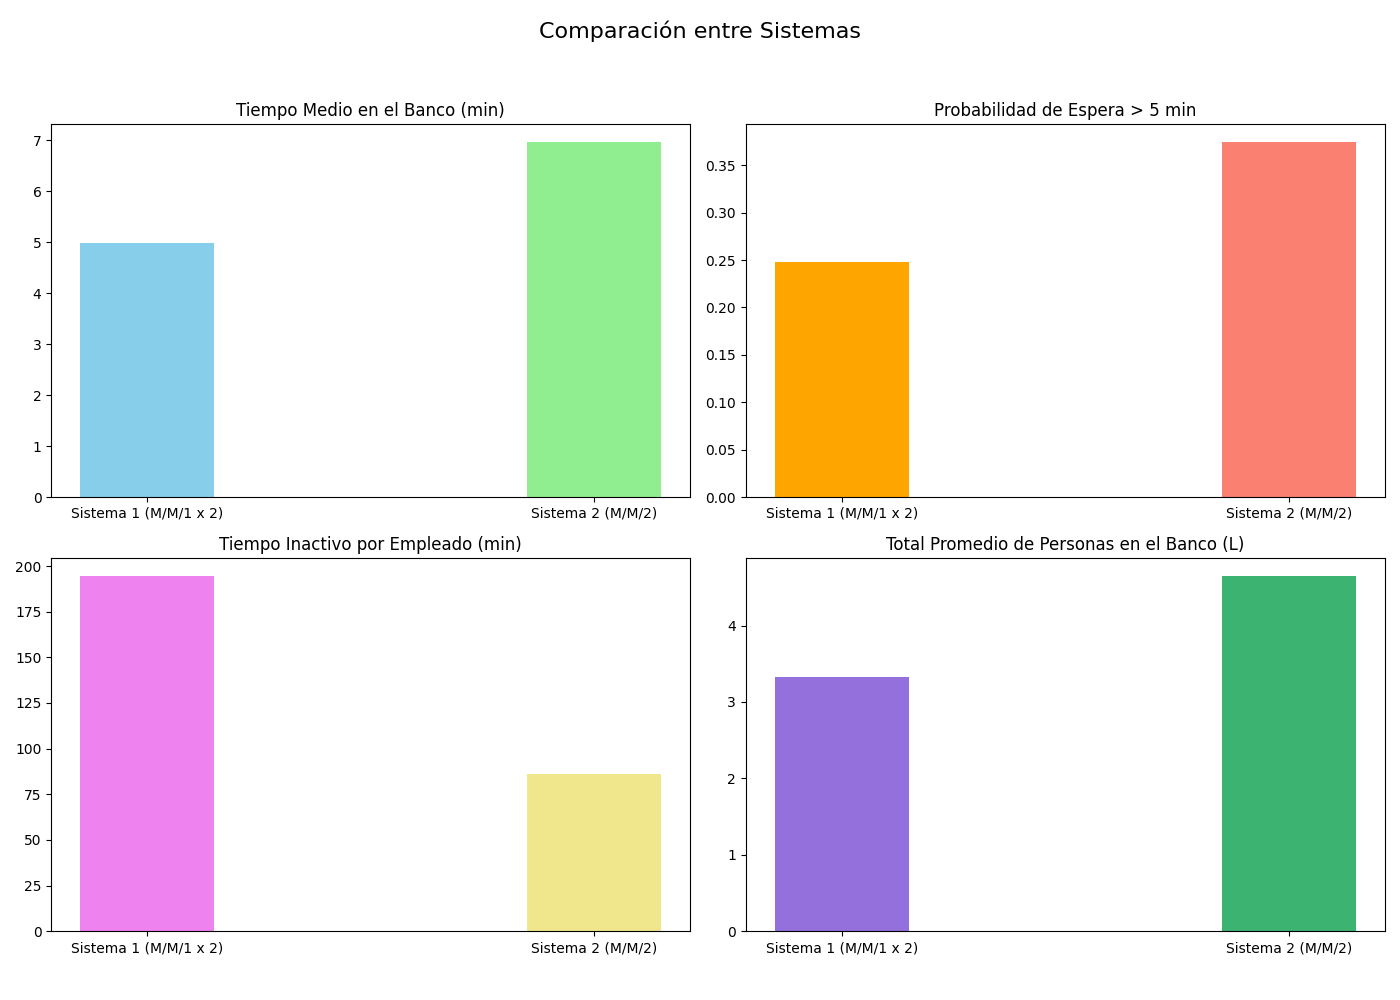
\includegraphics[width=0.9\textwidth]{../graphs/comparacion.png}
    \caption{Comparación entre los dos sistemas de atención}
    \label{fig:comparacion}
\end{figure}


\section{Conclusiones}\label{sec:conclusiones}
El análisis comparativo demuestra que:
\begin{itemize}
    \item El \textbf{sistema actual} (dos colas independientes) presenta una mayor eficiencia en términos de tiempo medio y menor número de clientes en el sistema, aunque a costa de una mayor inactividad por empleado.
    \item El \textbf{sistema propuesto} (cola única con dos servidores) ofrece mayor flexibilidad operativa, ya que evita la saturación desigual de las colas, aunque con un leve incremento en el tiempo de servicio (debido al aumento de la media de servicio a 2.4 minutos).
    \item La elección entre ambos sistemas dependerá de las prioridades operativas: eficiencia vs. equidad y experiencia del cliente.
\end{itemize}

\vfill

\end{document}
